\documentclass[a4paper,10pt]{article}
\usepackage[utf8]{inputenc}
\usepackage{graphicx}
\title{Towards best practices for a visualization chatbot}
\author{Maria Ferman}

\begin{document}

\maketitle
% interface-platform
% Rapid prototyping and conversational flow https://www.behance.net/gallery/37453869/Designing-a-Chatbot-UX-Design-Process-Case-Study
It is necessary to make software customized and accessible for users who do not have any technological background. Fortunately, chatbots can help with both issues. Chatbots allow users, through their own words, to interact and communicate with software. Therefore, software can become easier to understand and use. The efficiency of the chatbots can be augmented by considering the user preferences. By doing this, software can adapt to their preferences. According to Shevat,  ``Bots are a new user interface which lets users interact with services and brands using their favorite messaging apps. Bots are a new way to expose software through a conversational interface"~\cite{Shevat2017}. 

In order to make the interaction between the user and the chatbot more efficient, designers required a comprehensive list of best practices in chatbot's design. 
The design of a chatbot is more effective when the designers use specific practices that allows them not to start from scratch, but to give them a specific structure of how to design an efficient chatbot. 

\section*{Objective}

%Develop a set of best practices that allow designers to create and design a text-base chatbot. 
%To develop best practices for a visualization chatbot (Peggy)

To design and develop a chatbot in order to help novice users to create visualizations that allows them to analyse their data and discover deeper insights. The design of the chatbot will be carried out by developing a set of best practices that allow designers to efficiently create a text-based chatbot.  

\section*{Motivation}

%To help designers to effectively create chatbots by having a complete and accurate set of best practices. This best practices will allow users to have a specific guide (steps) about the chatbot's creation. The best practices will describe the necessary elements that integrate chatbot.     

%How to create designers to have more effective visualizations X chatbot  
%to help visualization users novices from the designer point of view - best practices help them 

Understanding data can be a difficult process for people without experience for creating visualizations. For example, project managers need to extract insights and discover patters in their data, and this may not be a straightforward process by using an excel table. Visualizations makes easy for novices understand their data. However, creating visualization is also a complicated task for novice people. Chatbots can help in the visualization creation and data analysis process. By interacting with a chatbot, novices can get help or an additional support for the visualization creation and visual data exploration.

However, people who create chatbots may have troubles to find a complete set of best practices to create and design a chatbot. This makes the chatbot creation process complicated and time consuming. Therefore, by having a complete and accurate set of best practices, help designers to effectively create chatbots. These best practices will allow users to have a specific guide (steps) about the chatbot's creation. The best practices will describe the necessary elements that integrate chatbot.     

%1.- Problema
%2.- Porque los gyidelines son necesarios
%3.- Trabajo previo, pero tal .. peor por esta razon ellos no solucionan el problema  

\section*{Project Description}

The project consists of three main phases. \textbf{The first phase} is the design of a Chatbot's best practices. In order to develop a good set of best practices, it will be necessary to read blogs and best practices online. Besides of selecting and using the most popular chatbots. 

\textbf{The second phase} is the muck-up of a visualization chatbot designed according to the best practices of the first phase, the visualization interface will be mimicked by using the Wizard of Oz simulation technique. According to Hutchby~\cite{Hutchby2001} \textit{Wizard of Oz} is a technique that involves humans masquerading as computer systems which are in the process of development, while the users recruited to test the "system" are led to believe that it is actually a computer with which they are interacting.  The simulation is used as a test-bed in which ideas about how the system should operated, as well as how humans may interact with the system, can be explored by designers." 

Finally, \textbf{the third phase} is the case study. This study will be carried out to evaluate the chatbot best practices. Therefore, if the chatbot fulfil the user requirements in the case study, this is a clear indication that the best practices are adequate for the creation of a chatbot.

% the chatbots' efficiency in interaction with the users in order to create effective visualizations.
 %PROJECT LIMITATIONS
 %The limitation is that it is subjective, it iwll take more time to fully validate it. 
 
Throughout the project I will use two different user-personas (Laura and Patricia). The creation of the two personas will guide me in the creation of these best practices, and to help me in the design of the chatbot. Finally, the personas will help me in the case study to select users that are close to the description of the project user-personas. 
% I am developing the creation of 

%PARAGRAPH TO DESCRIBE THE TWO DIFFERENT PERSONAS. 
The first user-persona is oriented to the Chatbot's best practices (Figure \ref{FigurePatricia}). Patricia is a developer who works in a startup company in Victoria, BC. She holds a Computer Science degree and has good programming skills. However, Patricia does not have experience designing chatbots. She lacks skills and knowledge on software design, and she has little time and lacks of motivation to read blogs and best practices online. In addition, she finds the amount of chatbots blogs overwhelming. Therefore, her goal is to find a set of guidelines that help her to design a chatbot effectively. 

The second user-persona is oriented to the chatbot (Figure \ref{FigureLaura}). Laura is a Visualization novice who works as a project manager in a mid-sized company in Victoria, BC. She has managed several projects successfully. However, she does not have any background creating visualizations. On a daily basis, she uses her computer, iPad, and mobile phone to work. She has problems in creating visualizations to explain her ideas and project results. She has little time to devote in the visualization creation process, and struggles in learning new technologies. Besides, she finds the amount of visualization tools overwhelming. Laura would like to find a good way, by using her mobile phone, to create an effective visualization. In addition, she would like to get help in the visualization creation and data analysis process.  
\begin{figure}
\centering
\includegraphics[scale=0.4]{/Users/MariaFerman/Desktop/ToRead(Project:Bots)/LaTexImages/BestPracticesPersona.png}
\caption{Best Practices' Persona}
\label{FigurePatricia}
\end{figure}

\textbf{Chatbot Best Practices' Design:} The best practices are created to allow people like Patricia to design an effective chatbot. These best practices give developers the most important aspects about the chatbot's design. Therefore, from the beginning they will have a specific structure to follow of how to design their chatbot (Figure \ref{FigureBestPracticeDiagram}). 

\begin{figure}
\centering
\includegraphics[scale=0.4]{/Users/MariaFerman/Desktop/ToRead(Project:Bots)/LaTexImages/PersonaProject.png}
\caption{Chatbot's Persona}
\label{FigureLaura}
\end{figure}

\textbf{Chatbot:} The goal of the chatbot is to help people like Laura to create a meaningful visualization about their data. Laura can use natural language statements in order to communicate with the chatbot. In response, the chatbot will provide her with several visualization options.

%Alexey's feedback: (on Visualizations: to communicate or to explore the data) 
\textbf{Chatbot's Tasks on Visualization:} The Visualization goal of the chatbot is to help users to analyse data by using visual context images (graphs). The chatbot will offer different options to visualize data. The options will be oriented to allow users to see patterns, trends, and correlations that might be not detected by the use of data tables or excel sheets. Therefore, the chatbot will allow users to easily analyse their data in order to have deeper insights.  

\begin{figure}[p]
    \makebox[\linewidth]{
        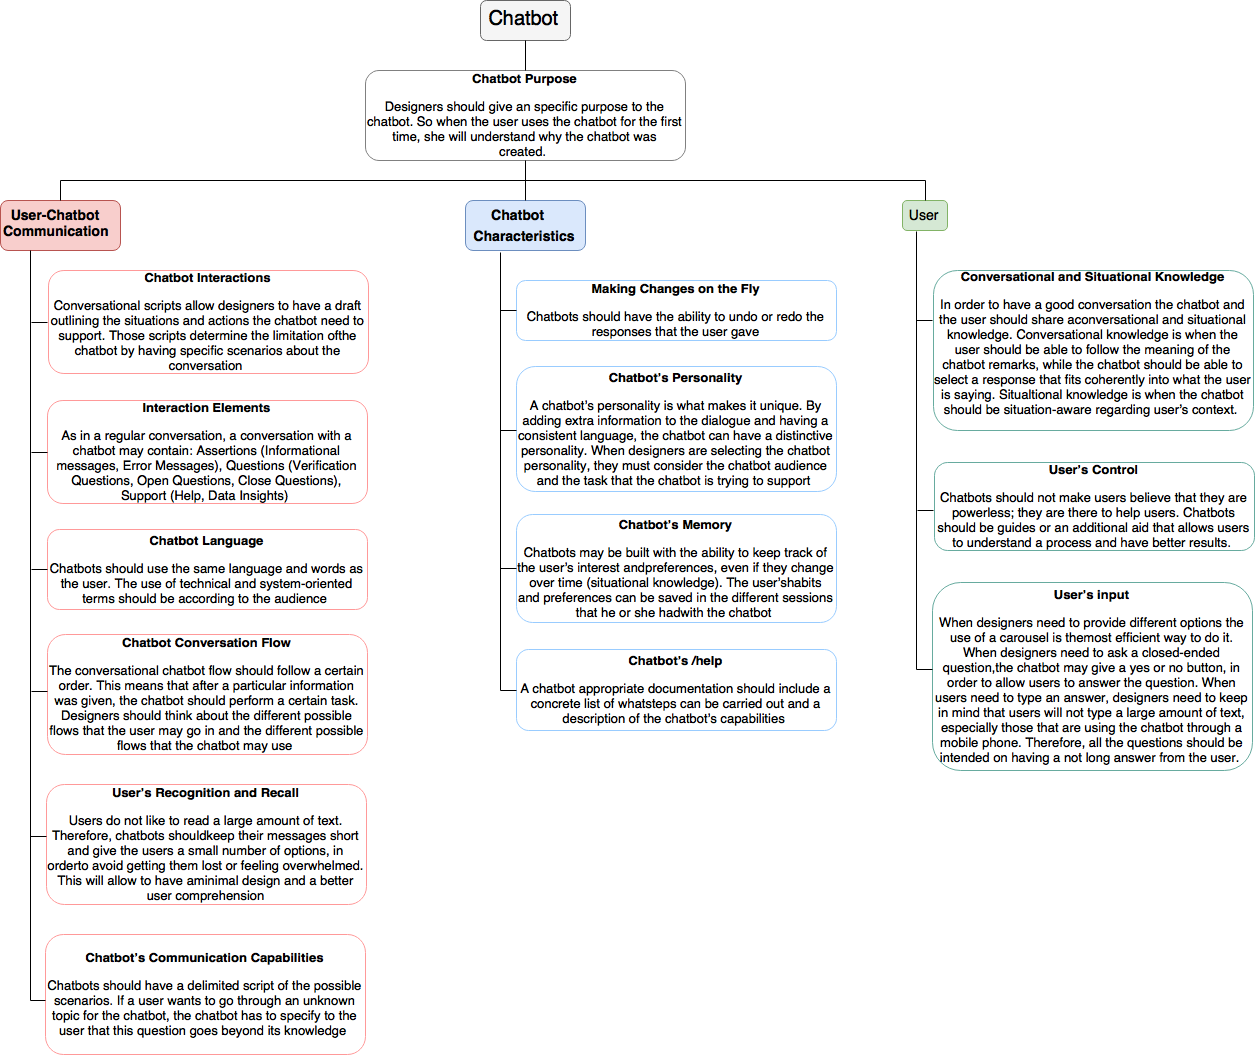
\includegraphics[width=1.6\linewidth]{/Users/MariaFerman/Desktop/ToRead(Project:Bots)/imgDesignfesst/BestPracticesDiagram.png}
    }
    \caption{Best Practices Diagram}
    \label{FigureBestPracticeDiagram}
\end{figure}


\newpage
\section{Chatbot Purpose}

The purpose of a chatbot should be clear to its users. A chatbot that makes a user feel confused about its purpose is futile. \textbf{Users need to have a clear understanding of why the chatbot was designed and what its capabilities and limitations are.}

Currently, chatbots' designers can deal with this issue in two different ways. The first is to have a clear explanation about the chatbot's capabilities at the beginning of the interaction with the users. A clear example of a chatbot purpose definition is the CNN chatbot (Figure \ref{FigurePurpose}). When the user opens the chatbot for the first time, the chabot describes him or her the top stories and gives an explanation about how to get more news according to his or her preferences. The second option is to allow users to discover by themselves the purpose and capabilities of the chatbot during the interaction.

Chatbot designers need to identify a balance between the constraints of the interface and the goals of users that they want to accomplish. Besides this, the kind of chatbot needed should be decided based on the final user's requirements, and if it is feasible to create them or not. After finding this balance and making this analysis, the designers should define what the chatbot's capabilities will be (i.e., what the chatbot can do in order to help users in their tasks). 

In addition, designers should understand when to use a direct manipulation interface (e.g., graphic user interface) and when to use a chatbot. Usually, conversational agents that do not have a clear purpose make the user feel that the job can be done by a regular website. Chatbots can be very useful as long as they are well-developed and oriented to the purpose.  

 %According with Maes \cite{shneiderman1997direct}, if a designer wants to create an agent that will work and has the trust of the user, it is important to understand  

\begin{figure}
\centering
\includegraphics[scale=0.4]{/Users/MariaFerman/Desktop/ToRead(Project:Bots)/LaTexImages/CNN_chatbot_purpose.png}
\caption{CNN Chatbot}
\label{FigurePurpose}
\end{figure}

% I
\section*{User-Chatbot Communication}

\section{Chatbot Interactions}

According to the Merriam-Webster dictionary, interaction is defined as the action or influence of things on one another \cite{merriam-webster}.
%According to the Cambridge dictionary, interaction is defined as the occasion when two or more people or things communicate with or react to each other!!!!!.
Chatbots should have a well-designed series of interactions with users. Every single intended interaction should have a specific script of the different conversations that the chatbot and the users may have. 

\textbf{\textit{Conversational scripts}} \textbf{allow users to have a ``draft outlining the situation and actions the chatbot need to support"~\cite{CaseStudy}. Those scripts determine the limitation of the chatbot by having specific scenarios about the conversation.} 

The most important and complex part of designing a chatbot is the creation of the conversational script, because the user can take many paths (conversation scenarios) in order to achieve one task~\cite{designChatbotConversatio}. In other words, users can select different paths which should all arrive at the same destination. One effective way to create those different scenarios is using mind maps. According to Eppler~\cite{eppler2006comparison}, ``Mind maps are defined as a a multicoloured and image centred, radial diagram that represents semantic or other connections between portions of learned material hierarchically." Figure \ref{FigureMindMap} shows a mind map regarding the different conversational scenarios of a chatbot that allow novice users to create visualizations. 

%\begin{figure}
%\includegraphics[scale=0.23]{/Users/MariaFerman/Desktop/ToRead(Project:Bots)/imgDesignfesst/ConversationalMindMap.png}
%\caption{Visualization Chatbot's Conversational Mind Map}
%\label{FigureMindMap}
%\end{figure}

\begin{figure}
    \makebox[\linewidth]{
        \includegraphics[width=1.7\linewidth]{/Users/MariaFerman/Desktop/ToRead(Project:Bots)/imgDesignfesst/ConversationalMindMap.png}
    }
    \caption{Visualization Chatbot's Conversational Mind Map}
   \label{FigureMindMap}
\end{figure}

After creating the mind maps, designers may use tools like InVision \footnote{www.invisionapp.com} in order to create the conversational chatbot mockups.

As in a human conversation, chatbots and users can have the same parts of a conversation such as greetings,  conversation and farewell.

\subsection{Greeting}
From the first interaction between a user and a chatbot, the users should have a clear idea of the chatbot context and what they can expect from it. Therefore, users should know the context in which the chatbot need to be used.

The welcome or greeting section is the first interaction in which chatbots should clearly communicate what they are capable of doing, in order to avoid functionality misunderstandings. 
%According to Lurchenko, the information in the welcome screen should not exceed 160 characters~\cite{CheatSheet}. 
The welcome section of the conversation should be short and concise, to avoid users feeling overwhelmed due to the amount of information provided by the chatbot. The first section of the figure \ref{FigureMindMap} shows the \textit{greeting conversational script} for a Visualization chatbot. This section shows the possibles greetings that a user may utilize for starting the conversation with the chatbot.  

\subsection{Conversation}
The conversation section is when the topic will be developed. According to Mishra ~\cite{effectivCommunication}, ``Effective communication is getting the message across as intended and getting desired feedback by influencing and attracting attention". Therefore, chatbots should be able to express a clear message to the user in order to have an effective communication. This section can have assertions, questions, comments, and feedback. The participants of the conversation should take turns interacting in order to communicate a clear message. A conversation with a visualization chatbot may have the following sections: \textit{Visualizations, More visualizations, Help, Refactoring, Undo, and Non-supported expressions} (Figure \ref{FigureMindMap}).

\subsection{Farewell}
The farewell section is the last part of a conversation. By this phase, the users should have had the help that they need in order to finish their task and to have relevant feedback. In this section, the chatbot should ask the user if the provided information or help was useful, and if the user would like to do anything else. The last section of the figure \ref{FigureMindMap} shows the \textit{farewell conversational script} for a Visualization chatbot. 
%------------------------------------------------------------------------------------------------------------------------------------------------------

\section{Interaction Elements}
According to Allen et al.~\cite{allen1978conversation}, \textbf{the speaker can emit several elements, such as assertions, questions, and support in a conversation.}Chatbots can emit the same elements (table \ref{InteractionElementsTable}). The following interaction elements are described from the chatbot's perspective. 

%https://www.socialresearchmethods.net/kb/questype.php

\begin{table}[]
\centering
\begin{tabular}{lllll}
\hline
\textbf{Assertions}    & \textbf{Questions}     & \textbf{Support}   \\
\hline
Informational messages & Verification Questions & Help      \\
Error Messages         & Open-ended Questions         & Data Insights.  \\
Warning Messages                       & Close-ended Questions        &       \\
Result Messages                       & Questions Based on Level Of Measurement       &       \\
Options                       & Contingency Questions       &       \\    
                       & Dichotomous Questions       &       \\  
     \hline                   
\end{tabular}
\caption{Interaction elements}
%\refstepcounter
\label{InteractionElementsTable}
\end{table}

\subsection{Assertions}
Assertions are affirmations or messages that the chatbot gives to the user; assertions determine the content of the conversation and allow the listener to increase his or her knowledge about a certain topic. 

\subsection{Questions}
Questions can be used to make sure that the provided information is required by the user. An example is when Poncho, the weather forecasts chatbot, asks users about the city for which they want to know the weather. If the user would like to know the weather in Manhattan, Poncho will ask the following verification question, ``New York, NY? Right now it's mostly cloudy there. Is that the right city?" and after the user click "yes" Poncho will give the complete forecast.(Figure \ref{FigureVerificationQuestion}).

%Open and close questions: https://robinhq.com/customer-service-guide/human-conversation/

\begin{figure}
\centering
\includegraphics[scale=0.3]{/Users/MariaFerman/Desktop/ToRead(Project:Bots)/imgDesignfesst/VerificationQuestion.png}
\caption{Poncho Weather Forecast Chatbot}
\label{FigureVerificationQuestion}
\end{figure}

However, designers should avoid open-ended questions, because users may respond in a non-supported way. A solution for this may be the use of questions that provide different options in buttons inside the chatbot message, and the chatbot should ask users to select one. Each provided option will invoke different actions. If the options provided by the chatbot contain several images, a good way to display them is the use of carousels. 

According to Pernice~\cite{carousel}, ``Carousels enable more than one piece of content to occupy the same piece of prime real estate on the homepage, which can help diffuse any infighting about whose content is most deserving" and it should not be included more than five frames in each carousel because it is hard for users to remember more than five topics at the same time. 

%to be include?
%To add Persistent menus - menus that are in teh interface not in the bot. always available information.  
% https://chatbotsmagazine.com/cheat-sheet-all-facebook-chatbot-interactions-4b14e4e00178

\subsection{Support}
Finally, support is any extra help that the chatbot gives to the user. This help should be straightforward for users. Commonly, users only need to type the word ``\textit{help}" or the command ``\textit{/help}" in order to get an additional support from the chatbot. When an error has occurred the chatbot should automatically ask users if they need any help. Besides, chatbots can also give feedback as a part of the conversational support, or provide meaningful insights about the performed task or the conversation that the user and the chatbot had.\\[0\baselineskip] In addition, users should be able to ask for extra information at any point in the conversational flow.
\\
\\
Besides regular human conversational elements, chatbots may understand command expressions. These statements are commands that users with a domain specific knowledge use to interact with the chatbot.

%\section{Conversational Script}
%The conversational script should take into account the following elements: timing, being an active participant and an active listener, and avoiding over sharing information.

%The chatbot's messages elements can include text, emojis, attached files, images, video or audio. The message can be structured; these types of messages follow the command line format and usually have buttons to allow users to get information or to answer a question previously asked by the chatbot. The content of the message should be short in order to have a minimal design and a better user comprehension.  %According to Lurchenko the content of the buttons should not exceed 20 characters including spaces~\cite{CheatSheet}. Besides, the font of the message should be in an adequate size, besides it can have bold, italic, fixed-width text, and inline links. 
%------------------------------------------------------------------------------------------------------------------------------------------------------
\section{Chatbot Language}
According to Allen et al.~\cite{allen1978conversation}, in order to have a meaningful conversation, it is necessary to share a language and have vocabulary in common. \textbf{Chatbots should use the same language and words as the user. The use of technical and system-oriented terms should be according to the audience.} 

 If the design of the conversational agent is oriented to certain populations, chatbots can mimic how users normally speak.  Therefore, before the creation of the chatbot, it is necessary to have a ``solid understanding of the audience we seek to appeal to, and to have a vocabulary familiar to them”~\cite{HeuristicsWebPage}. Figure \ref{FigureIRIS} shows a conversation between a user and Iris\footnote{https://github.com/Ejhfast/iris-agent/}, the data science chatbot. Iris is oriented to a scientific audience, therefore the language, that Iris uses, is according to a domain specific area.  

\begin{figure}
\centering
\includegraphics[scale=0.4]{/Users/MariaFerman/Desktop/ToRead(Project:Bots)/imgDesignfesst/IRIS-image.png}
\caption{Iris Data Science Chatbot}
\label{FigureIRIS}
\end{figure}
%------------------------------------------------------------------------------------------------------------------------------------------------------
\section{Chatbot Conversation Flow}
According to Reichman~\cite{reichman1985getting}, in a usual conversation many details are being shared. To avoid an incoherent conversational flow, it is necessary that listeners understand when and why the conversational topic has been changed. \textbf{The conversational chatbot flow should follow a certain order. This means that after a particular information was given, the chatbot should perform a certain task.} 

\textbf{Designers should think about the different possible flows that the user may go in and the different possible flows that the chatbot may use.} Users and chatbots can change the topic of the conversation at any point. Shifting the conversation topic should be made carefully to avoid misunderstandings. For example, ShopBot\footnote{https://shopbot.ebay.com/} from Ebay helps users to select a pair of jeans, and after selecting the desired jeans, the user can also ask for a blouse from a different department (Figure \ref{FigureEbay}). It is important to understand that the purpose of the conversation did not change, the purpose remains the same (buying clothes). However, the flow of the conversation switch from buying jeans to blouses from a different department.
%Another example is Poncho, users can ask him about the weather, and then change the conversation's topic and have a little chat with Poncho about astrology. 

\begin{figure}
\centering
\includegraphics[scale=0.5]{/Users/MariaFerman/Desktop/ToRead(Project:Bots)/imgDesignfesst/ShopBot.png}
\caption{ShopBot Ebay}
\label{FigureEbay}
\end{figure}

%* For instance, the design of the chatbots can twist the conversation from talking about a certain graph and when the user has selected the graph, to what color is better to use /find another example/. Shifting the conversation topic should be made carefully to avoid misunderstandings.  * 

Chatbots may change the flow of a conversation according to the chatbot purpose. An example of this is Rescue.io (Figure \ref{FigureRescue}). This chatbot was created to aim emergency situations. "During an emergency when the user cannot phone someone for help, Rescue can quickly alert the user's emergency contacts to what is happening and where the user is so they can help"~\cite{Rescue}. Rescue will lead the conversational flow by asking a series of questions about the type of emergency that the user has. 

\begin{figure}
\centering
\includegraphics[scale=0.5]{/Users/MariaFerman/Desktop/ToRead(Project:Bots)/imgDesignfesst/rescued.png}
\caption{Rescue Emergency Chat Service}
\label{FigureRescue}
\end{figure}

Chatbots need to follow a conversational script that is a structured development of the conversation, to avoid references that are not clear to the participants, and engage users in the conversation.(?after move)

The conversation between the user and the chatbot should not lead to any ambiguity about what to say in the conversation. Therefore, the chatbot's conversation should be structured and have messages that are clear and concise. By using structured conversation, chatbots can guide a user through the interaction~\cite{HeuristicsWebPage}.(?after move)

%However, designers should be careful of not letting the chatbot lose the feeling of a normal conversation. Some conversations might be structured too rigidly; for this reason they seem to be a command line, instead of giving the user the conversational feeling that chatbots should have. The flow of the conversation should be natural and evident. 
%------------------------------------------------------------------------------------------------------------------------------------------------------
\section{User's Recognition and Recall}

According to Scott, \textbf{users do not like to read a large amount of text: ``they will read the first message and then their eyes glaze over. They skim the rest of the text”}~\cite{HeuristicsWebPage}. The principle of least effort, set forth by Zipf, also specifies that people use shortened words and expression in speech, in order to obtain the maximum communication by using the least cost~\cite{zipf2016human}. \textbf{Therefore, chatbots should keep their messages short and give the users a small number of options, in order to avoid users getting lost or feeling overwhelmed. This will allow to have a minimal design and a better user comprehension.}

In addition, users do not remember details of the options given by an interface. When users avoid reading a large amount of text, they may misunderstand the chatbot’s message and finish with an unsuccessful result. The design of the chatbot dialogue should only have relevant information to help users with their tasks and prevent a dull interaction with the chatbot. 
%... p.8
%------------------------------------------------------------------------------------------------------------------------------------------------------

\section{Chatbot's Communication Capabilities}

\textbf{Chatbots should have a delimited script of the possible scenarios (Figure \ref{FigureMindMap}). If a user wants to go through an unknown topic for the chatbot, the chatbot has to specify to the user that this question goes beyond its knowledge.} For example, when a user asks Poncho, the weather chatbot, something that it was not created to answer, Poncho replies with: ``Oops, I didn't catch that. For things I can help you with, type \textit{help}"~\cite{HeuristicsWebPage} (Figure \ref{FigureCommunicationCapabilities}). Chatbots need to gracefully establish limits to users that want to go beyond the chatbot's knowledge.  

\begin{figure}
\centering
\includegraphics[scale=0.4]{/Users/MariaFerman/Desktop/ToRead(Project:Bots)/imgDesignfesst/PonchoHelp.png}
\caption{Poncho Weather Forecast Chatbot}
\label{FigureCommunicationCapabilities}
\end{figure}
%------------------------------------------------------------------------------------------------------------------------------------------------------

% II
\section*{Chatbot Characteristics}

\section{Chatbot's Personality}

The Oxford dictionary defines personality as the combination of characteristics or qualities that form an individual's distinctive character~\cite{Oxford}. \textbf{A chatbot’s personality is what makes a chatbot unique. By adding extra information to the dialogue and having a matching language, the chatbot can have a distinctive personality.} However, designers should be careful to not include too much additional information that makes the user feel bored or annoyed. There has to be a balance between giving just the relevant information and adding extra information to make the chatbot's conversation more engaging. Therefore, the chatbot personality is an important part to make the user more engaged with the interface.

The chatbot’s personality should take into account the target audience for which it was designed. The personality should match with the users: therefore, how friendly, sarcastic or humorous should only depend on the people who will use the chatbot. Therefore, \textbf{when designers are selecting the chatbot personality, they must consider the chatbot audience and the task that the chatbot is trying to support.}  

Users like to interact with chatbots in a human way~\cite{HeuristicsWebPage}. For this reason designers should consider how to engage users in the conversation. 

A clear example of how to get user engagement is the Aura's Bot\footnote{http://m.me/aurapower}. Aura Dione is a Danish singer who is using a chatbot in order to be in contact with her fans. The designer of the Aura's Bot uses the personality of the singer. (Figure \ref{FigureAura}). Therefore, the tone of the chatbot is like an artist, and fans can communicate with it and ask extra information about the singer. Fans have the feeling of interacting with the singer, and this leads to the user engagement and retention~\cite{personality}.  

\begin{figure}
\centering
\includegraphics[scale=0.5]{/Users/MariaFerman/Desktop/ToRead(Project:Bots)/imgDesignfesst/AuraBot.png}
\caption{Aura's Bot}
\label{FigureAura}
\end{figure}

According to Scott~\cite{HeuristicsWebPage}, there is a difference between the content (\textit{relevant information to help the user}) and the medium (\textit{the chatbot’s personality}). Users need to be entertained and at the same time to be helped.      

%Spectrm establishes a series of questions in order to select the right personality for a chatbot: ``Do you have a mascot (for a product or brand)? Does this mascot have a personality that might serve as inspiration? Is there a core value for your company in general or to its way of communication that could inspire the personality? Can you think of a person you know, a celebrity or a fictional character that your bot could resemble?" \cite{personality}. Those questions allow designers to create a template or structure about how they want the chatbot to behave and interact with the users.

Other important considerations to take into account are the age, heritage, friends and occupation that the chatbot may have. All these specifications enable designers to have a clear definition of whom the chatbot will resemble.

To summarize, the chatbot’s success may be defined by how designers balance between entertainment and guidance. Therefore, the difference between chatbots that are being used and those that are not, is how compelling and pleasant the chatbot experience is.

%\section{Chatbot's Audience - Should be a subsection of Personality?}

%Chatbots can be developed for business, customer oriented tasks, or just be oriented to teen customers~\cite{Shevat2017}. Business oriented tasks' chatbots are designed to help teams to collaborate in a more effective way. This kind of chatbots can be useful to help software developers in their task because ``it can help reduce the friction points they have to face when working collaboratively"~\cite{lebeuf2017software}. An example of a business oriented task chatbot is the slackbot\footnote{https://api.slack.com}. The consumer oriented tasks' chatbots are designed to help users communicate, get additional information or help. An example is Poncho the weather forecast chatbot. Finally, the teen oriented chatbots are developed to entertain young customers and these kinds of users like to play games, chat and share content with friends. An example of this chatbot is Kik\footnote{https://bots.kik.com/}. 

%According to Shevat, in order to define the chatbot's audience, developers need to answer the following questions: Are you addressing a business use case? Is this a consumer use case? Are you targeting teens? Families? Adults at work? When are they using the service? \cite{Shevat2017}.

%\section{Chatbot's Versatility}
%retrival base bots - question answer 
%Chatbots should be versatile enough to be able to understand open-questions, commands, and requests written by the user. An example of an open-question is when users ask Poncho, "What's the weather like in Brooklyn this weekend?" and then Poncho answers with the Brooklyn weather forecast. 

%However, if a user wants to use a command in the interaction with the chatbot, the dialogue should continue smoothly without breaking the flow. Commands to chatbots can be conveyed via special characters followed by an argument. For example, chatbots' commands in Slack and Telegram start with a slash follow by an argument. The characters of the argument can be Latin letters, numbers and underscores~\cite{botfather}. It is a common practice to have slash commands in the following pattern: slash ``command name" ``arguments"~\cite{Shevat2017}.  
%------------------------------------------------------------------------------------------------------------------------------------------------------
\section{Chatbot's Memory}

\textbf{Chatbots should be built with the ability to keep track of the user's interest and preferences, even if they change over time \textit{(situational knowledge)}. Conversational agents can save the user's habits and preferences in the different sessions that he or she had with the chatbot}~\cite{shneiderman1997direct}. As an example of this, Poncho can save the location of a certain user. Therefore, the next time that the user asks for a weather broadcast, Poncho already knows which location to look at, saving the user time and keystrokes. Besides, these allow the user to have a customised experience. 

%If I come back, Poncho will remember my location, saving me a few keystrokes.*
%------------------------------------------------------------------------------------------------------------------------------------------------------
\section{Making Corrections on the Fly}

It is normal that users make mistakes when they are choosing different options in an interface. \textbf{It is very important that chatbots have the ability to undo or redo users responses.} In that case, users know that they are able to undo an unwanted change triggered by a misinterpreted message or a mistaken click~\cite{HeuristicsWebPage}. %Therefore, designers must take into account that users may make mistakes. 
Figure \ref{FigureUndo} shows an example of a chatbot without the undo capability. In this example, the user made a mistake in the items added to the shopping cart. Because the chatbot does not have this ability, the user has two options, start the conversation from the beginning or buy all the items that are in the shopping cart even if he or she does not need them. This is a good example of why chatbots need to provide this functionality, because users will feel annoyed of starting the whole conversation again or may not be willing to purchase mistaken added items *. 

During a conversation, Chatbots have hints about when a user made a mistake. In the previous example, when the user said "I meant" is a clear indication of the user made a mistake. Therefore words as "meant" gives designers a clue of when to use the undo capability.

Another approach is that the chatbot directly asks users if the information provided is accurate. The Poncho chatbot has the ability to ask users if the information provided was appropriate; if not, users can clarify it.  

\begin{figure}
\centering
\includegraphics[scale=0.5]{/Users/MariaFerman/Desktop/ToRead(Project:Bots)/imgDesignfesst/Undo2.png}
\caption{Chatbot Without an Undo Capability}
\label{FigureUndo}
\end{figure}

%\section{Error Messages}

%Chatbots should express error messages in a straightforward way. They should not use codes or technical words to avoid confusing and stressing the user. Chatbots should be able to express that an error has occurred and add suggestions about how to solve or undo that error. 

%Error prevention allows users to understand that something unexpected just happened in the interaction. For example, an error can be a wrong input data from the user. In the case of such an event, the chatbot should allow users to get additional help or undo what they have just done. Some chatbots  allow to speak with a live agent in the event that the user is struggling with the chatbot interaction. An example of this is 1-800-Flowers Assistant~\footnote{https://www.facebook.com/1800FlowersAssistant/}, this conversational agent can connect a live agent if the conversation with the chatbot fallows for a certain period of time. 

%To summarize, a good chatbot should be able to provide evidence around error prevention and allow users to recover when an error just happened~\cite{HeuristicsWebPage}. 
%------------------------------------------------------------------------------------------------------------------------------------------------------
\section{Chatbot's /help}

Chatbots should be used without the need for extra information. How to use a chatbot should be a simple conversational flow. However, there are some users that like to deeply understand how the interface works and detect its limitations. \textbf{A chatbot appropriate documentation should be precise and short. It should provide extra information about how the chatbot can help users in their tasks.} Besides, it also should include a concrete list of what steps can be carried out and the critical points of the chatbot~\cite{HeuristicsWebPage}. 

Finally, the chatbot should provide an easy way to access the documentation. One example of this is when the user types slash ``/" and a list of the supported commands of the chatbot should appear on the screen~\cite{botfather}.  
%------------------------------------------------------------------------------------------------------------------------------------------------------

% III
\section*{User}

\section{Conversational and Situational Knowledge}

Conversations need to follow certain rules and to have a certain semantic order for the sake of having a clear understanding between the user and the chatbot. Therefore, in order to have a good conversation the chatbot and the user should share a conversational and situational knowledge. 

%The chatbot script should follow the same rules and semantic order as a regular conversation. In other words, there should be a mapping between the script and the actual conversation. Designers need to understand what the actual conversation will feel like for the users and then create the chatbot accordingly. 

\textbf{\textit{Conversational Knowledge}} \textbf{is when the user is able to follow the meaning of the chatbot's remarks, while the chatbot is able to select a response that fits coherently into what the user is saying.} Therefore, it is vital to understand how chatbots and users follow each others' thoughts. In other words, Conversational Knowledge is the common definitions in the conversation that do not change over time. 

Figure \ref{FigurePoncho} shows the user asking Poncho\footnote{https://poncho.is/} (the weather forecast chatbot) to have the temperature in Celsius rather than Fahrenheit degrees. In this example, the temperature units are the shared conversational knowledge. For this reason the user request makes sense in the conversational context, and the chatbot is able to make the conversion of the temperature.     


\textbf{\textit{Situational Knowledge}} is another important part of having a mutual understanding in a conversation. According to Reichman~\cite{reichman1985getting} people need to share Situational Knowledge in order to understand and follow a conversation because it involves previous knowledge about the topic that is being discussed.  

In a user-chatbot conversation, Situational Knowledge \textbf{is when the chatbot is situation-aware regarding the user context.} Therefore, Situational Knowledge change over time according to the user's context. Figure \ref{FigurePoncho} shows a user asking "What is the temperature in London right now? Due to Poncho and the user share the same situational knowledge about the current time, the provided forecast will be according to the time, when the user asked the information. 

%Listeners must be able to follow the context of the conversation; they need to grasp what the speaker's point is and what he or she said before. Listeners need to understand the prior and the current context of the conversation to avoid being confused and to grasp the conversation's assertion. At the same time, speakers need to follow the order of a conversation to make their remarks easily understandable to the listeners. Therefore, the user and the chatbot should \textit{share the same information, to be on the same page.} 

\begin{figure}
\centering
\includegraphics[scale=0.2]{/Users/MariaFerman/Desktop/ToRead(Project:Bots)/imgDesignfesst/PonchoConversationLines.png}
\caption{Poncho Weather Forecast Chatbot}
\label{FigurePoncho}
\end{figure}
%------------------------------------------------------------------------------------------------------------------------------------------------------
\section{User's Control}

Users are accustomed to and like having control over the software. For instance, when a user has the ability of doing more customizations in an interface, they tend to feel more engaged in using that interface, because it has the user preferences. Therefore, it is extremely important to make the user feel that he or she has control over the interface. According to Maes~\cite{shneiderman1997direct}, ``users must be able to to turn over control of task to conversational agents but users must never feel out of control".

\textbf{Chatbots should not make users believe that they are powerless over the interface; they are there to help users to have a better experience using the interface. Chatbots should be guides or an additional aid that allows users to understand the interface and have better results.} According to Shneiderman~\cite{shneiderman1997direct}, it is ``necessary to give the users the feeling of being in control and therefore they can be responsible for the decisions they make.” 
%------------------------------------------------------------------------------------------------------------------------------------------------------
\section{User's input}

\textbf{There are several ways that the chatbot may receive the input from a user, by clicking an image in a carousel, clicking buttons or by directly typing a message in a text box, among others.} And designers need to have a clear understanding about when is a better option for users to click rather than type. 

When chatbots need to provide different options, from which the user need to select one, the use of a carousel is the most efficient way. When chatbots need to ask a closed-ended question, the chatbot may give a yes or no button, in order to allow users to answer the question. When users need to type an open-ended answer, designers need to keep in mind that users will not type a large amount of text, especially those that are using the chatbot through a mobile phone. Therefore, all the questions should be intended on having a not long answer from the user. Besides, it is also difficult for the chatbot to understand the user's intent from a long paragraph. 
%------------------------------------------------------------------------------------------------------------------------------------------------------

Autonomy of the bots, Interaction between the bots and the player, and the bots’ Presence in the game world. The work in [11] also implicates personality, emotion, self-motivation, the illusion of life (which includes goals, plans, reactions to the environment, human-like restrictions, and many other behaviours which create the appearance of life), change, and social relationships as being important to character believability. This supports the commonly referenced definition of believability proposed by Loyall [40].

Personality in agents is defined as the agent’s pattern of behav- iours or interactions with its environment [37]

\medskip

\bibliographystyle{unsrt}%Used BibTeX style is unsrt
\bibliography{References.bib}

\end{document}